\section{Refleksion}

\begin{frame}
\frametitle{I hvilken kontekst er smartphonen?}
\begin{figure}
\centering

\begin{minipage}{\textwidth}
        \begin{subfigure}[b]{0.3\textwidth}
                \includegraphics[width=\textwidth]{graphics/smartphone_on_table}
                \caption{Smartphone på et natbord.}
                \label{context:table}
        \end{subfigure}
        ~ %add desired spacing between images, e. g. ~, \quad, \qquad, \hfill etc.
          %(or a blank line to force the subfigure onto a new line)
        \begin{subfigure}[b]{0.3\textwidth}
                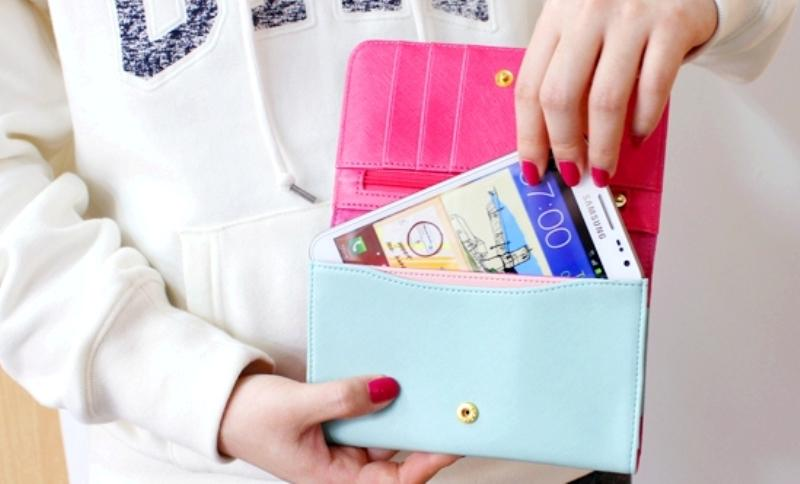
\includegraphics[width=\textwidth]{graphics/smartphone_in_purse}
                \caption{Smartphone i en taske.}
                \label{context:purse}
        \end{subfigure}
        ~ %add desired spacing between images, e. g. ~, \quad, \qquad, \hfill etc.
          %(or a blank line to force the subfigure onto a new line)
        \begin{subfigure}[b]{0.3\textwidth}
                
\includegraphics[width=\textwidth]{graphics/swimmer}
                \caption{Når man fx er ude at svømme.}
                \label{context:swimmer}
        \end{subfigure}
\end{minipage}
\begin{minipage}{\textwidth}
	\begin{subfigure}[b]{0.3\textwidth}
		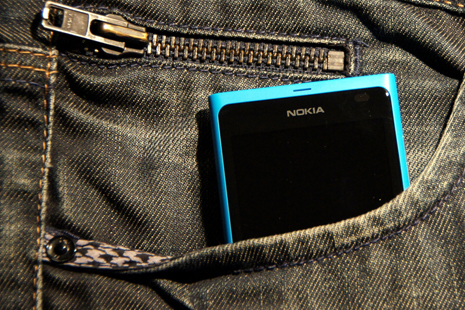
\includegraphics[width=\textwidth]{graphics/smartphone_pocket}
		\caption{Smartphone i lommen.}
		\label{context:pocket}
		\end{subfigure}
		~ %add desired spacing between images, e. g. ~, \quad, \qquad, \hfill etc.
		%(or a blank line to force the subfigure onto a new line)
		\begin{subfigure}[b]{0.3\textwidth}
			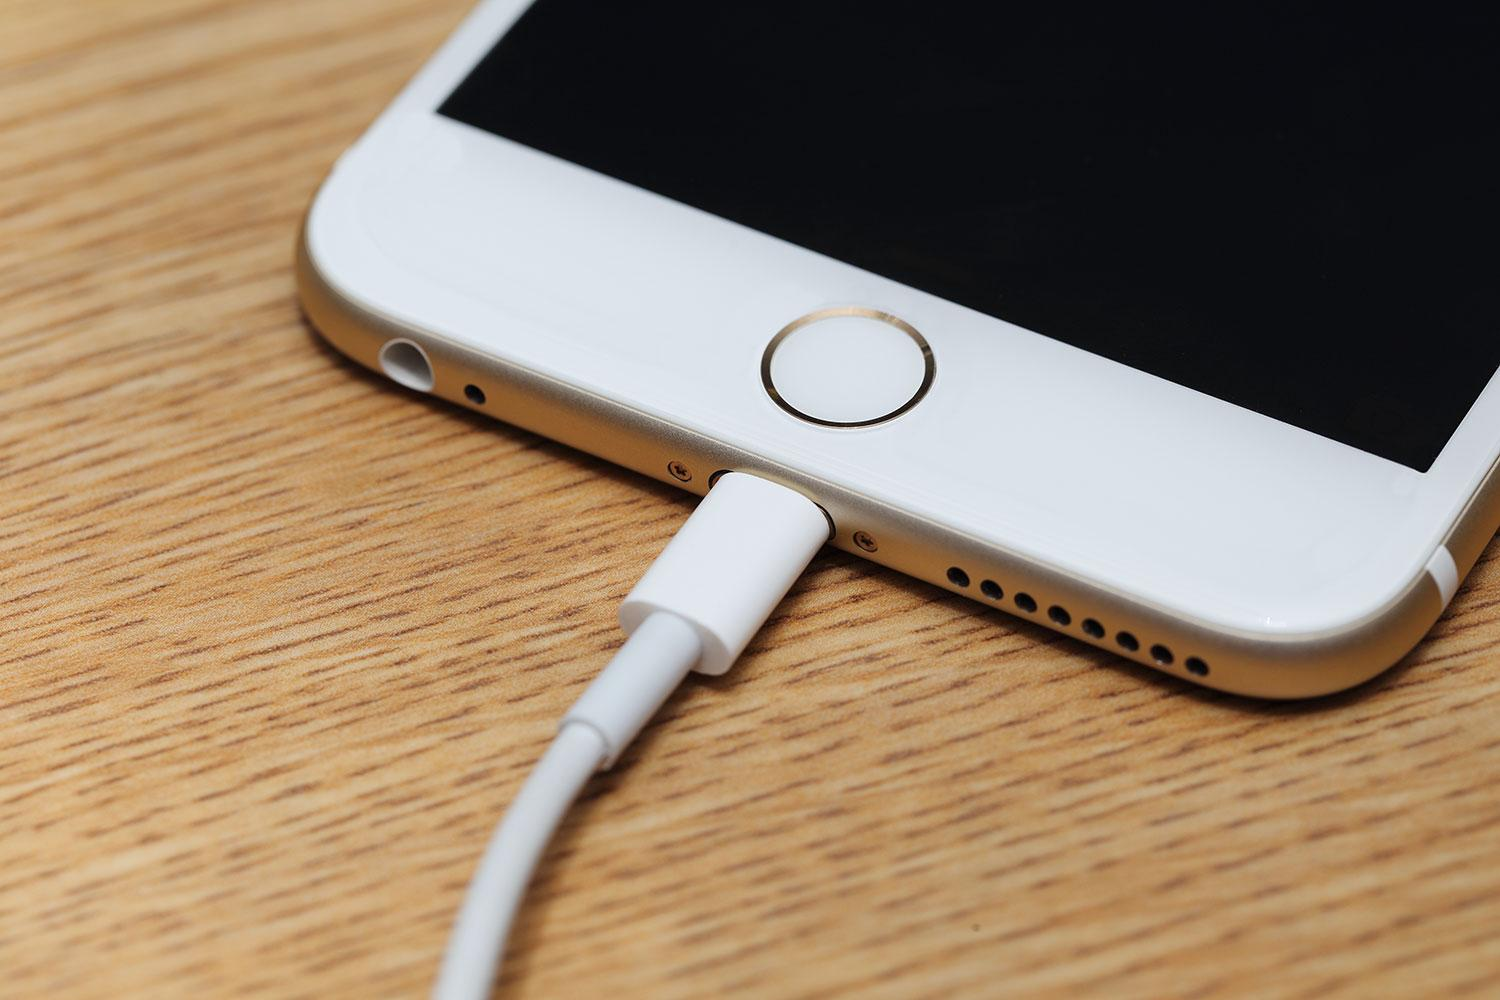
\includegraphics[width=\textwidth]{graphics/smartphone_charging}
			\caption{Smartphone til opladning.}
			\label{context:charging}
			\end{subfigure}
			~ %add desired spacing between images, e. g. ~, \quad, \qquad, \hfill etc.
			%(or a blank line to force the subfigure onto a new line)
			\begin{subfigure}[b]{0.3\textwidth}
				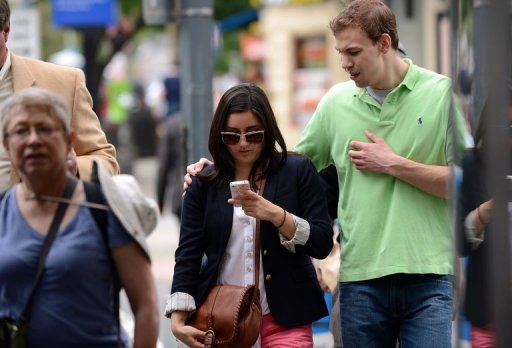
\includegraphics[width=\textwidth]{graphics/smartphone_other_user}
				\caption{Smartphone bruges af en anden.}
				\label{context:other_user}
				\end{subfigure}
\end{minipage}
\label{context}

\end{figure}
\end{frame}

\begin{frame}
\frametitle{Notifikationer}
\begin{itemize}
\item På baggrund af fokusgruppeinterviewet er notifikationer en god ide
\item En status for patienten
\begin{itemize}
\item Notifikationer der direkte fortæller om fremgang eller tilbagegang
\item Tidsinterval	
\end{itemize}

\item Eller 'refleksionsnotifikationer': Fx at patienten har en dårlig søvnrytmne eller ikke snakker med så mange mennesker som han plejer	
\item Patienten vælger selv notifikationer
\end{itemize}
\end{frame}

\begin{frame}
\frametitle{Huskekort}
\begin{itemize}
\item Et huskekort bruges i pressede situationer
\begin{itemize}
	\item En presset situation kan være når patienten oplever tilbagegang
\end{itemize}
\item Et huskekort er en liste af ting som er aftalt med behandeleren
\begin{itemize}
	\item Det kan fx være lystbetonede aktiviteter eller et mobilnummer til en kontaktperson
\end{itemize} 
\item Huskekort kan implementeres som notifikationer
\end{itemize}
\end{frame}

\begin{frame}
\frametitle{Dataindsamling}
Pladsmangel kan være et problem, her er nogle mulige løsninger:
\begin{itemize}
\item Gemme data i skyen(Giver ingen komplikationer for arkitekturen)
\item Komprimere data
\item Lavere opdateringshastighed på sensorer
\item Direkte forbindelse mellem moduler, så man ikke behøver at lagre i databasen
\end{itemize}
\end{frame}

\begin{frame}
\frametitle{Databaserettigheder}
Alle moduler kan skrive til alle database tabeller, det kan være et problem.
Mulig løsning:
\begin{itemize}
\item Manageren opretter en nøgle for et modul som skal bruges for at tilgå dens databasetabeller
\end{itemize}
\end{frame}

\begin{frame}
	\frametitle{Nøgleudveksling: Nyt modul}
	\begin{tikzpicture}[
	>=stealth,
	node distance=3cm,
	database/.style={
		cylinder,
		cylinder uses custom fill,
		cylinder body fill=yellow!50,
		cylinder end fill=yellow!50,
		shape border rotate=90,
		aspect=0.25,
		draw
		}
		]
		\node[database] (db1) at (1,2) {Keys};
		
		\draw  (-5,3) rectangle (-1,1);
		\draw  (-5,0) rectangle (-1,-2);
		\draw  (0,3) rectangle (4,1);
		\node at (-4,-1) {Module: A};
		\node at (-4,2) {Manager};
		\node at (3,2) {DB Access};
		\node at (-4,-0.5) {New};
		\end{tikzpicture}
\end{frame}

\begin{frame}
	\frametitle{Nøgleudveksling: Nyt modul}
	\begin{tikzpicture}[
	>=stealth,
	node distance=3cm,
	database/.style={
		cylinder,
		cylinder uses custom fill,
		cylinder body fill=yellow!50,
		cylinder end fill=yellow!50,
		shape border rotate=90,
		aspect=0.25,
		draw
	}
	]
	\node[database] (db1) at (1,2) {Keys};
	
	\draw  (-5,3) rectangle (-1,1);
	\draw  (-5,0) rectangle (-1,-2);
	\draw  (0,3) rectangle (4,1);
	\node at (-4,-1) {Module: A};
	\node at (-4,2) {Manager};
	\node at (3,2) {DB Access};
	\node (v1) at (-2,2) {$K_a$};
	\node at (-4,-0.5) {New};
	\end{tikzpicture}
\end{frame}

\begin{frame}
	\frametitle{Nøgleudveksling: Nyt modul}
	\begin{tikzpicture}[
	>=stealth,
	node distance=3cm,
	database/.style={
		cylinder,
		cylinder uses custom fill,
		cylinder body fill=yellow!50,
		cylinder end fill=yellow!50,
		shape border rotate=90,
		aspect=0.25,
		draw
	}
	]
	\node[database] (db1) at (1,2) {Keys};
	
	\draw  (-5,3) rectangle (-1,1);
	\draw  (-5,0) rectangle (-1,-2);
	\draw  (0,3) rectangle (4,1);
	\node at (-4,-1) {Module: A};
	\node at (-4,2) {Manager};
	\node at (3,2) {DB Access};
	\node (v1) at (-2,2) {$K_a$};
	\node (v2) at (-2,-1) {$K_a$};
	\draw [->] (v1) edge (v2);
	\node at (-4,-0.5) {New};
	\end{tikzpicture}
\end{frame}

\begin{frame}
	\frametitle{Nøgleudveksling: Nyt modul}
	\begin{tikzpicture}[
	>=stealth,
	node distance=3cm,
	database/.style={
		cylinder,
		cylinder uses custom fill,
		cylinder body fill=yellow!50,
		cylinder end fill=yellow!50,
		shape border rotate=90,
		aspect=0.25,
		draw
	}
	]
	\node[database] (db1) at (1,2) {Keys};
	
	\draw  (-5,3) rectangle (-1,1);
	\draw  (-5,0) rectangle (-1,-2);
	\draw  (0,3) rectangle (4,1);
	\node at (-4,-1) {Module: A};
	\node at (-4,2) {Manager};
	\node at (3,2) {DB Access};
	\node (v1) at (-2,2) {$K_a$};
	\node (v2) at (-2,-1) {$K_a$};
	\draw [->] (v1) edge (db1);
	\draw [->] (v1) edge (v2);
	\node at (-4,-0.5) {New};
	\end{tikzpicture}
\end{frame}

\begin{frame}
	\frametitle{Nøgleudveksling: Skriv til DB}
	\begin{tikzpicture}[
	>=stealth,
	node distance=3cm,
	database/.style={
		cylinder,
		cylinder uses custom fill,
		cylinder body fill=yellow!50,
		cylinder end fill=yellow!50,
		shape border rotate=90,
		aspect=0.25,
		draw
	}
	]
	\node[database] (db1) at (1,-1) {Keys};
	\node[database] (db2) at (2,-4) {DB};
	
	
	\draw  (-5,0) rectangle (-2,-2);
	\draw  (0,0) rectangle (4,-2);
	\node at (-4,-1) {Module: A};
	
	\node at (3,-1) {DB Access};
	
	\node (v2) at (-2.5,-1) {$K_a$};
	
	\node at (-1,-0.8) {write($K_a$)};
	\node at (2.5,-2.8) {write};
	\node (v1) at (-2,-1) {};
	\node (v3) at (0,-1) {};
	\draw[->] (v1) edge (v3);
	\node (v4) at (2,-2) {};
	\draw[->]  (v4) edge (db2);
	\end{tikzpicture}
\end{frame}

\section{Afrunding}
\begin{frame}
\frametitle{Individuelle projekter/moduler}
Ud fra denne platform er der arbejdet med to projekter der omhandler søvn og social aktivitet.
\end{frame}
